\documentclass{article}
\usepackage[utf8]{inputenc}
\usepackage[greek,english]{babel}
\usepackage{alphabeta}
\usepackage{fancyhdr}
\usepackage{listings}
\usepackage{mathtools}
\usepackage{xcolor}
\usepackage{biblatex}
\usepackage[left=2cm,right=2cm]{geometry}

\lstset {
        basicstyle=\ttfamily,
        columns=fullflexible,
        breaklines=true,
        keepspaces=true
}

\title{Σχεδίαση Ψηφιακών Συστημάτων - Εργασία Θεωρίας (Μέρος 3)}
\author{Χρήστος Μαργιώλης}
\date{Ιούλιος 2020}

\begin{document}

\begin{titlepage}
        \maketitle
\end{titlepage}

\renewcommand{\contentsname}{Περιεχόμενα}
\tableofcontents

\section{Κώδικας και τεκμηρίωση}

\subsection{\lstinline{alu_ctrl.vhd}}

Το παρακάτω κύκλωμα υλοποιεί την μονάδα ελέγχου της ALU. Ο τρόπος υλοποιήσης
της αρχικτεκτονικής προκύπτει από τους πίνακες λειτουργίας που υπάρχουνε στην
εκφώνηση της άσκησης και στις διαφάνειες του μαθήματος. Το κύκλωμα θα μπορούσε
να υλοποιηθεί εναλλακτικά χρησιμοποιώντας την δομή \lstinline{with-select} ή την
\lstinline{case}. \\

\lstinputlisting[language=VHDL]{../alu_ctrl.vhd}
\pagebreak

\subsection{\lstinline{alu_ctrl_tb.vhd}}

Στο παρακάτω testbench δοκιμάζουμε την μονάδα ελέγχου ALU δίνοντας τις τιμές
που υπάρχουνε στην εκφώνηση της άσκησης. \\

\lstinputlisting[language=VHDL]{../alu_ctrl_tb.vhd}
\pagebreak

\subsection{\lstinline{alu_ctrl_test_alu.vhd}}

Το παρακάτω κύκλωμα υλοποιεί ένα «δοκιμαστικό» κύκλωμα για την ALU και την μονάδα
ελέγχου της. Το μόνο που χρειάζεται είναι απλώς να δηλώσουμε ως components την ALU
που δημιουργήθηκε στο μέρος 1 και το προηγούμενο κύκλωμα, και να τα κάνουμε
map στα κατάλληλα πεδία του entity του κυκλώματος. Αυτή τη φορά, η αρχιτεκτονική 
θα είναι structural. \\

\lstinputlisting[language=VHDL]{../alu_ctrl_test_alu.vhd}
\pagebreak

\subsection{\lstinline{alu_ctrl_test_alu_tb.vhd}}

Testbench για το παραπάνω κύκλωμα. \\

\lstinputlisting[language=VHDL]{../alu_ctrl_test_alu_tb.vhd}
\pagebreak

\section{Εκτέλεση}

\subsection{\lstinline{alu_ctrl_tb}}
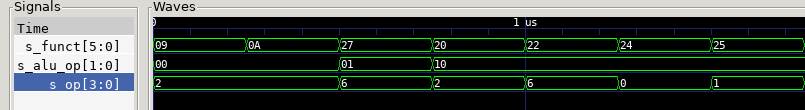
\includegraphics[width=\textwidth]{res/alu_ctrl.png}

\subsection{\lstinline{alu_ctrl_test_alu_tb}}
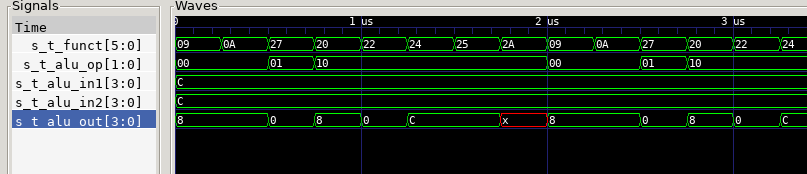
\includegraphics[width=\textwidth]{res/alu_ctrl_test_alu.png}

\end{document}
